
%
% LaTeX report template 
%
\documentclass[a4paper,10pt]{article}
\usepackage{graphicx}
\usepackage[english]{babel}
\usepackage[utf8]{inputenc}
\usepackage[T1]{fontenc}
%\usepackage{apacite}
\usepackage{float}
\usepackage[section]{placeins}
\usepackage{mwe}
\bibliographystyle{apalike}
\usepackage{hyperref}
\usepackage{mathtools}

\begin{document}
%
   \title{Rapport de stage PHIMECA}

   \author{Kristof Attila Simady \\ e-mail: kristof.simady@sigma-clermont.fr}
          
   \date{05/03/2020}

   \maketitle
   
   \tableofcontents
 
  \newpage
    
\section*{Avant propos}
% When adding * to \section, \subsection, etc... LaTeX will not assign
% a number to the section
Le cadre d'étude offert par SIGMA Clermont à donné la possibilité d’effectuer
une année supplémentaire de stage pour étoffer nos connaissances scientifiques, 
et découvrir le monde industriel comme des cultures étrangères.
De par mon appétence pour la recherche et l'informatique, j'ai eu la chance de
pouvoir venir effectuer mon stage au sein de l'entreprise \textbf{PHIMECA}, 
située à Clermont-Ferrand, et depuis longtemps en partenariat avec SIGMA.

Ce stage aura été l'occasion pour moi ... (à suivre) 

Je souhaite remercier ... (à suivre)

\paragraph{Note:}
Ce document est autant un rapport de stage qu'une note à qui voudrait se 
servir des différentes méthodes explorées et codes développés.

\section{Introduction}
Dans le cadre d'analyse probabiliste et fiabiliste, il est d'usage d’effectuer 
des analyses de sensibilité sur une ou plusieurs grandeurs d’intérêt, grâce
à divers moyens comme les indices de Sobol' ou les analyses de corrélation. \\
Ces analyses sont néanmoins souvent cantonnées à des modèles n'ayant en sortie et entrée que des
grandeurs scalaires, pour lesquelles de nombreuses méthodes existent dans la littérature.\\
L'objectif du travail présenté ici, est d’effectuer ce type d'analyse sur des modèles ayant en entrée plusieurs champs aléatoires et des variables aléatoires scalaires et en sortie aussi des champs et grandeurs scalaires. \\ Pour compléter cela, il était bien sûr aussi demandé de d'abord créer un modèle simple gouverné par des champs stochastiques et de faire de l'analyse de sensibilité sur ce modèle. \\
Il sera d'abord présenté différentes méthodes présentes dans la littérature, avec leurs potentiels avantages et défauts. \\ 
Cette approche des l'analyse de sensibilité nous renvoie aussi sur des champs de recherche bien différents, car les méthodes peuvent autant venir du champ de la mécanique que de la géologie ou l'étude environnementale.

 
\section{Recherche bibliographique}
Ce travail de recherche a été l'occasion de parcourir un grand nombre de travaux, liés de plus ou moins loin à l'analyse de sensibilité sur des processus gaussiens.\\
On notera notamment les travaux de \cite{Lilburne2009Feb} qui donnent dans leur travail un état de l'art complet sur les différentes méthodes utilisables pour l'analyse de sensibilité sur champs gaussiens. \\
D'autres techniques plus récentes ont néanmoins vu le jour, et ce sont ces dernières que nous avons explorés en premier. Notamment les travaux de \cite{Wei2017May} sur l'analyse de sensibilité de structures ayant en entrée des variables aléatoires et processus stochastiques variant dans le temps, ou encore le travail de \cite{Pronzato2019Jul} qui développe un métamodel entre l'entrée et sortie d'un modèle gouverné par des champs stochastiques.

\subsection{Travaux retenus}
Etant donné que les missions d'analyse de sensibilité et d'incertitudes se font classiquement en se basant sur la bibliothèque \textit{openTURNS} développé par PHIMECA, le choix a été fait d'adapter techniques de recherche et méthodes déja existantes dans l'API au problème étudié. 


\subsection{Methodes et outils de travail}
L'ensemblde des codes ont été écrits dans le langage \textit{Python}, en se servant majoritairement des bibliothèques a caractère scientifique (\textit{SciPy, NumPy}) et la bibliothèque développée en partie par \textbf{PHIMECA :} \textit{openTURNS} (\emph{open treatment of Uncertainties and Risk \& Statistics })\cite{OpenTURNS}.\\
\textbf{PHIMECA} a fourni un poste de travail Linux, tout comme un accès au serveur de calcul pour les modèles un peu plus conséquents. \\

\subsection[Prémices]{Analyse de la problématique, premier tests et prise en main des outils}

\subsubsection{Mission confiée et tâches associées}
L'objectif du stage était de développer une méthodologie pour l'analyse de sensibilité sur des modèles gouvernés par des champs aléatoires (Champs Stochastiques) et des variables aléatoires, et qui en sortie sont aussi représentables par une collection de champs et variables aléatoires. \\
Plus spécifiquement, cette méthodologie était à appliquer à un modèle d'échangeur de chaleur air-air commercialisé par \textbf{LIEBHERR} et utilisé pour la régulation thermique de l'air ambiant dans les avions de ligne.\\\\
Comme la mission confiée au sein de \textbf{PHIMECA} se rapprochait d'un travail de recherche, celui -ci était bien sur accompagné de nombreuses étapes distinctes. En effet, en plus du développement des codes et de l'application analytique, une recherche bibliographique a du être menée en amont pour parvenir a lister les différentes méthodes d'analyse existantes et tester celles qui pourraient convenir au mieux. De plus, une phase d'apprentissage et de tests a du d'abord être nécessaire pour parvenir à prendre en main les différents outils, et comprendre la théorie et les mathématiques sous-jacentes.\\

\subsubsection{Prise en main d'openTURNS et de la théorie sur les champs stochastiques}
\paragraph{Champs Stochastiques\\} 
Un champ stochastique est un champ de variables aléatoires toutes corrélées entre elles, et dont l'intensité de la corrélation est déterminée par leur proximité dans l'espace. Par exemple la position de tout objet est corrélée à sa position aux intervalles de temps proches (continuité du temps), ou bien les températures au dessus d'un pays sont corrélés à faible distance mais l'effet aléatoire est plus présent lorsque les distances sont importantes. \\
Ce type de modélisation des champs est couramment utilisée pour modéliser des propriétés présentant des variabilités gaussiennes mais une continuité dans leur espace de définition. \\ Lorsque la corrélation est seulement dépendante de la distance entre deux points de l'espace et non d'une position absolue, on parle d'un champ stationnaire. Lors de cette étude, on se place dans ce cas.\\ 

\newpage

\begin{figure}[H]
   \centering   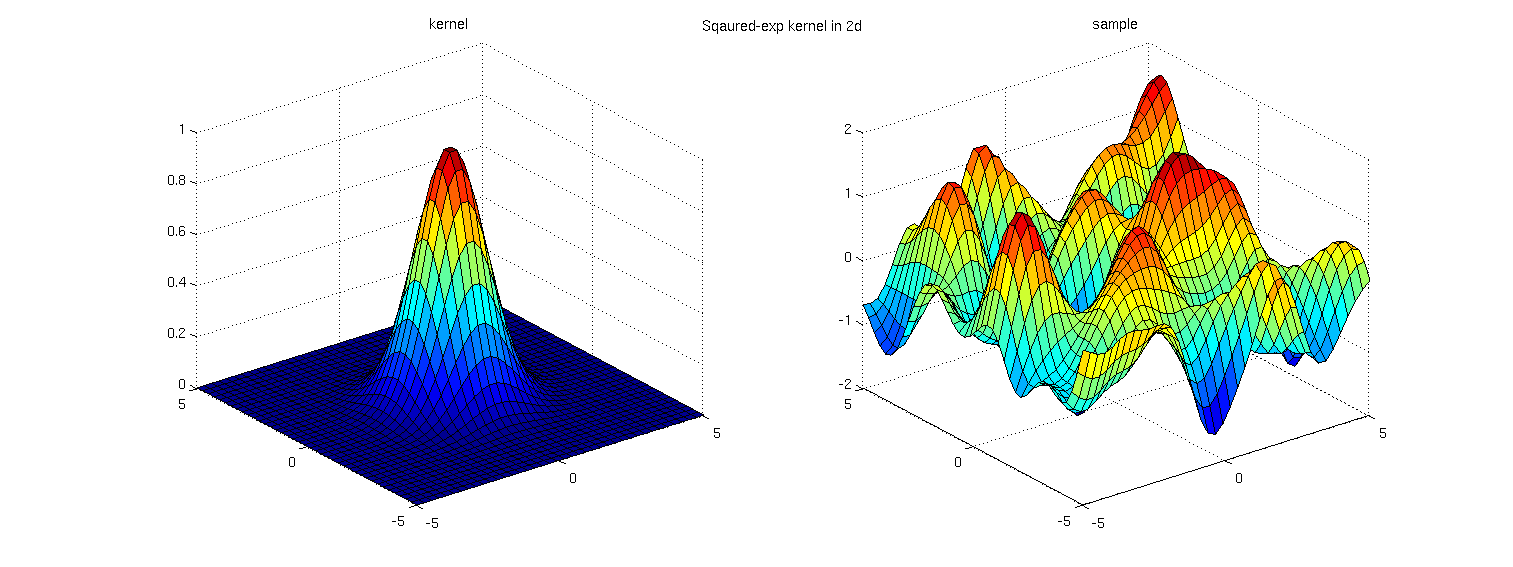
\includegraphics[scale=0.25]{stochastic_process2d.png}
      \caption{Réalisation d'un champ stochastique en deux dimension. Le champ est continu dans l'espace et la primitive est une gaussienne en deux dimensions.}
         \label{realChamp}
\end{figure}

Mathématiquement, cette corrélation peut être définie par différents modèles. Les deux modèles de corrélation les plus simples sont les fonctions de covariance exponentielles (1) et les exponentielles quadratiques (2).  

   \begin{eqnarray}
      				C(d) & = & \exp(-d/V)\\
                    C(d) & = & \exp(-(d/V)^{2});
   \end{eqnarray}
   
Avec \emph{V} étant le paramètre d'échelle et \emph{d} la norme euclidienne de la distance entre deux points de l'espace considéré.\textit{(plus le paramètre d'échelle est grand, plus le champ est lissé, tout comme le modèle quadratique est aussi plus lisse)}\\
Une autre fonction de covariance, celle de \emph{Matérn}, est aussi très utilisée, puisqu'elle présente des comportements limites similaires aux deux fonctions exponentielles présentes plus haut. La dérivabilité de ce modèle est réglable via le paramètre $\nu$, ainsi la régularité du champ est facilement modifiable.

   \begin{eqnarray}
C_{v}(d) & = & \sigma^{2}\frac{2^{1-\nu}}{\Gamma(\nu)}\left(\sqrt{2\nu}\frac{d}{\rho}\right)^{\nu}K_{\nu}\left(\sqrt{2\nu}\frac{d}{\rho}\right);
   \end{eqnarray}\\

La continuité des processus gaussiens et leur comportement quasi ondulaire, permet de les traiter de manière un peu analogue à la décomposition de fourrier, et des les décomposer en une somme infinie de variables aléatoires gaussiennes décorrélées.. Cette méthode de décomposition vient du théorème de \emph{Karhunen-Loève}. \\
La construction de cette série infinie se fait grâce aux vecteurs propres issus de la matrice de corrélation du modèle, et grâce à une base de vecteurs orthonormaux dans un espace Hilbertien. Les détails mathématiques de cette méthode peuvent être trouvées en  \cite{Sudret2000Jan}. \\
Lors de l’approximation de \emph{Karhunen-Loève}, la série est tronquée à l'ordre \textbf{M}.
%Approximation de Kahrunen Loeve 
   \[
      \begin{array}{lp{0.8\linewidth}}
         H(\textbf{x}, \theta) & Approx. Procéssus Gaussien \\
         \lambda_{i}          & Valeur Propre de la matrice de covariance \\
         \xi_{i}             & Variable Normale Centrée Réduite \\
         \varphi_{i}(\textbf{x}) & Vecteur propre de la matrice de covariance
      \end{array}
   \]
   \begin{eqnarray}
H(\textbf{x}, \theta) & = & \sum_{i=1}^{M}\sqrt{\lambda_{i}}\xi_{i}(\theta)\varphi_{i}(\textbf{x});
   \end{eqnarray}\\

Cette décomposition permet de représenter l'ensemble de variabilité du champ avec des variables gaussiennes décorrélées, et donc de faire des analyses de sensibilités sur cette nouvelle représentation du champ.

\paragraph{openTURNS\\}
\emph{openTURNS} est initialement un projet de bibliothèque open-source pour le traitement des incertitudes et des risques, commun a trois entreprises fondatrices, \textbf{Airbus}, \textbf{EDF} et \textbf{Phimeca Engineering}, projet ayant débuté en 2005. \\
Depuis, deux autres organismes, \textbf{IMACS} et l'\textbf{ONERA} ont rejoint le développement d'\emph{openTURNS}, qui se révèle être un grand atout pour le traitement des incertitudes et l’ingénierie fiabiliste.
En effet, le projet d'\emph{openTURNS} est un regroupement d'un ensemble d'algorithmes performants écrits en C++, se basant sur la théorie développée pour les traitement des incertitudes, l'optimisation robuste, et les études de sensibilité.\\ 
Un \textit{wrapper} a été utilisée pour lier l'ensemble de la bibliothèque C++ à un module Python, et de pouvoir profiter de la facilité d'utilisation du langage Python et de sa flexibilité, tout en gardant les vitesses d’exécution du C++.\\
\textbf{PHIMECA} développe des logiciels commerciaux en se basant sur le module \emph{openTURNS}, qui sont plus ergonomiques dans leur utilisation et automatisent certaines parties moins évidentes en utilisation directe de la librairie. \\
Néanmoins, la librairie reste quand même extrêmement bien documentée, avec la théorie mathématique sous-jacente à chaque algorithme d'explicitée, tout comme de nombreux exemples. La documentation présente de même des cas d'applications précis montrant la logique à avoir lors de l'écriture de codes avec \emph{openTURNS}.



\subsection{Exemple théorique simple, premiers codes}
Pour parvenir a tester les méthodes trouvées lors de la recherche bibliographique, et avoir un modèle simple et rapide à exécuter, un exemple simple a été développé : 
Il s'agit d'un modèle de poutre en appui sur ses deux extrémités
\begin{figure}[H]
   \centering   
   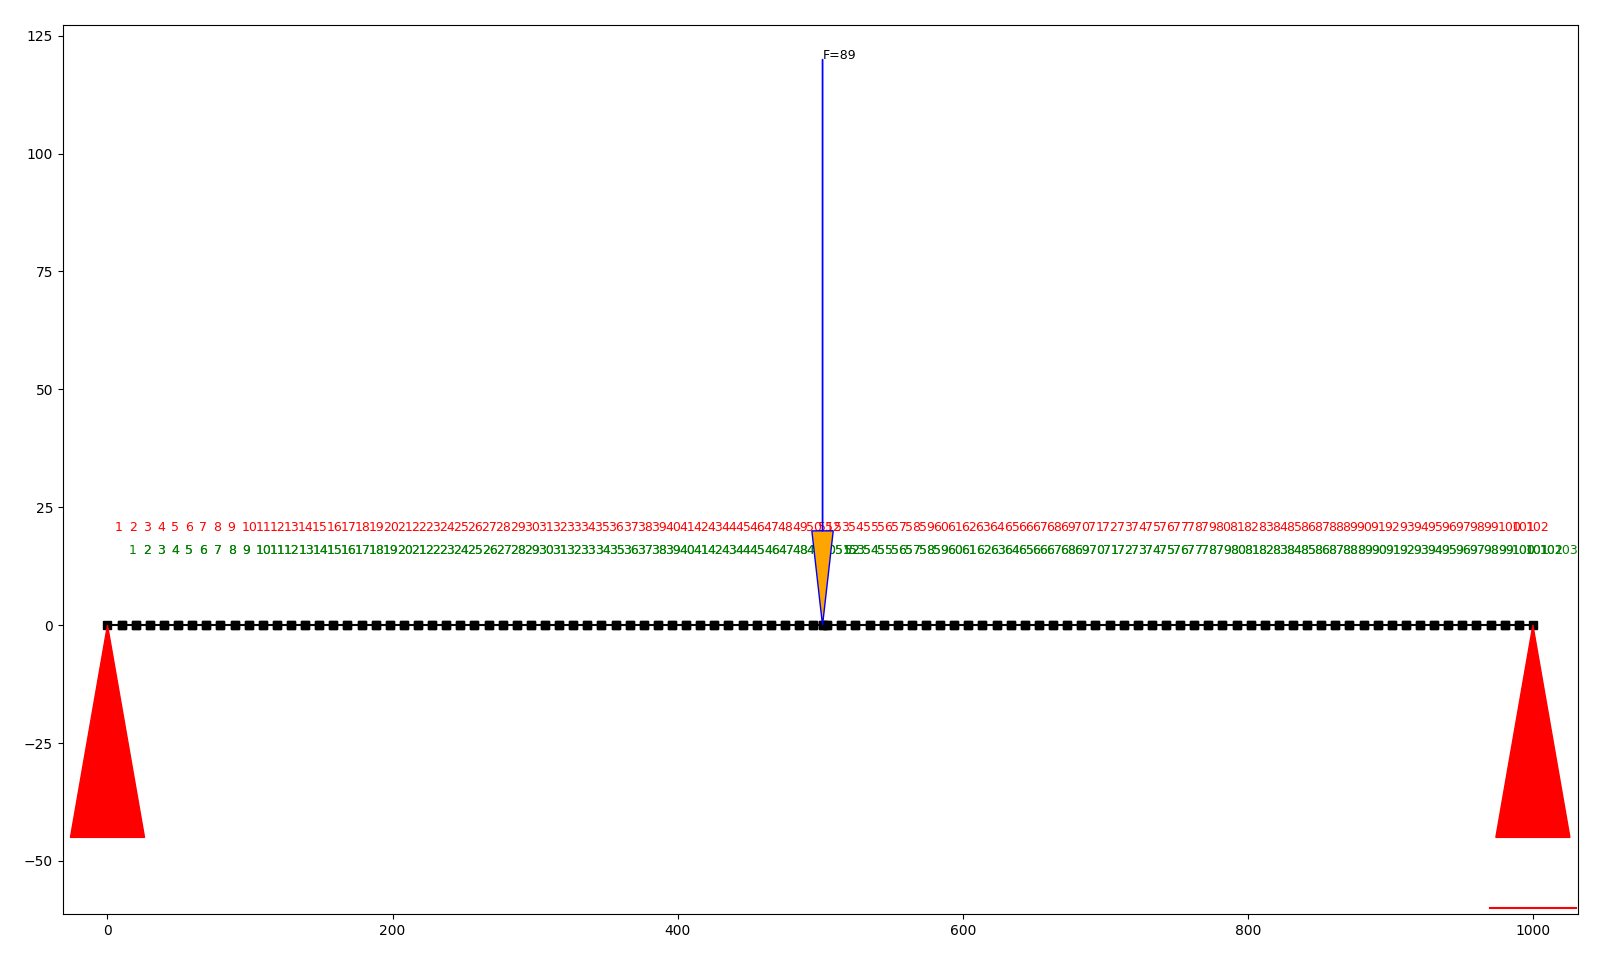
\includegraphics[scale=0.20]{beam_structure.png}
      \caption{Modélisation d'une poutre en appui sur ses deux extrémités avec la bibliothèque anastruct}
         \label{fig:nonfloat}
\end{figure}

La particularité de ce modèle de poutre est, en plus d'être une aberration physique, le fait que le diamètre et le module de young sont gouvernés par un processus gaussien en une dimension, suivant la longueur de la barre. Pour parvenir à modéliser cette variation, le modèle est bien-sûr subdivisé en une centaine d'éléments finis, et le champ discrétisé sur un maillage de même longueur.\\
En plus de ces deux grandeurs gouvernées par des champs, la densité du matériau, la position de la force, et la norme de la force sont représentés par des variables aléatoires Gaussiennes. Cette modélisations'est faite avec l'excellente bibliothèque \textbf{\textit{Anastruct}} de \cite{Vink2020Feb}.

\begin{figure}[H]
   \centering   
   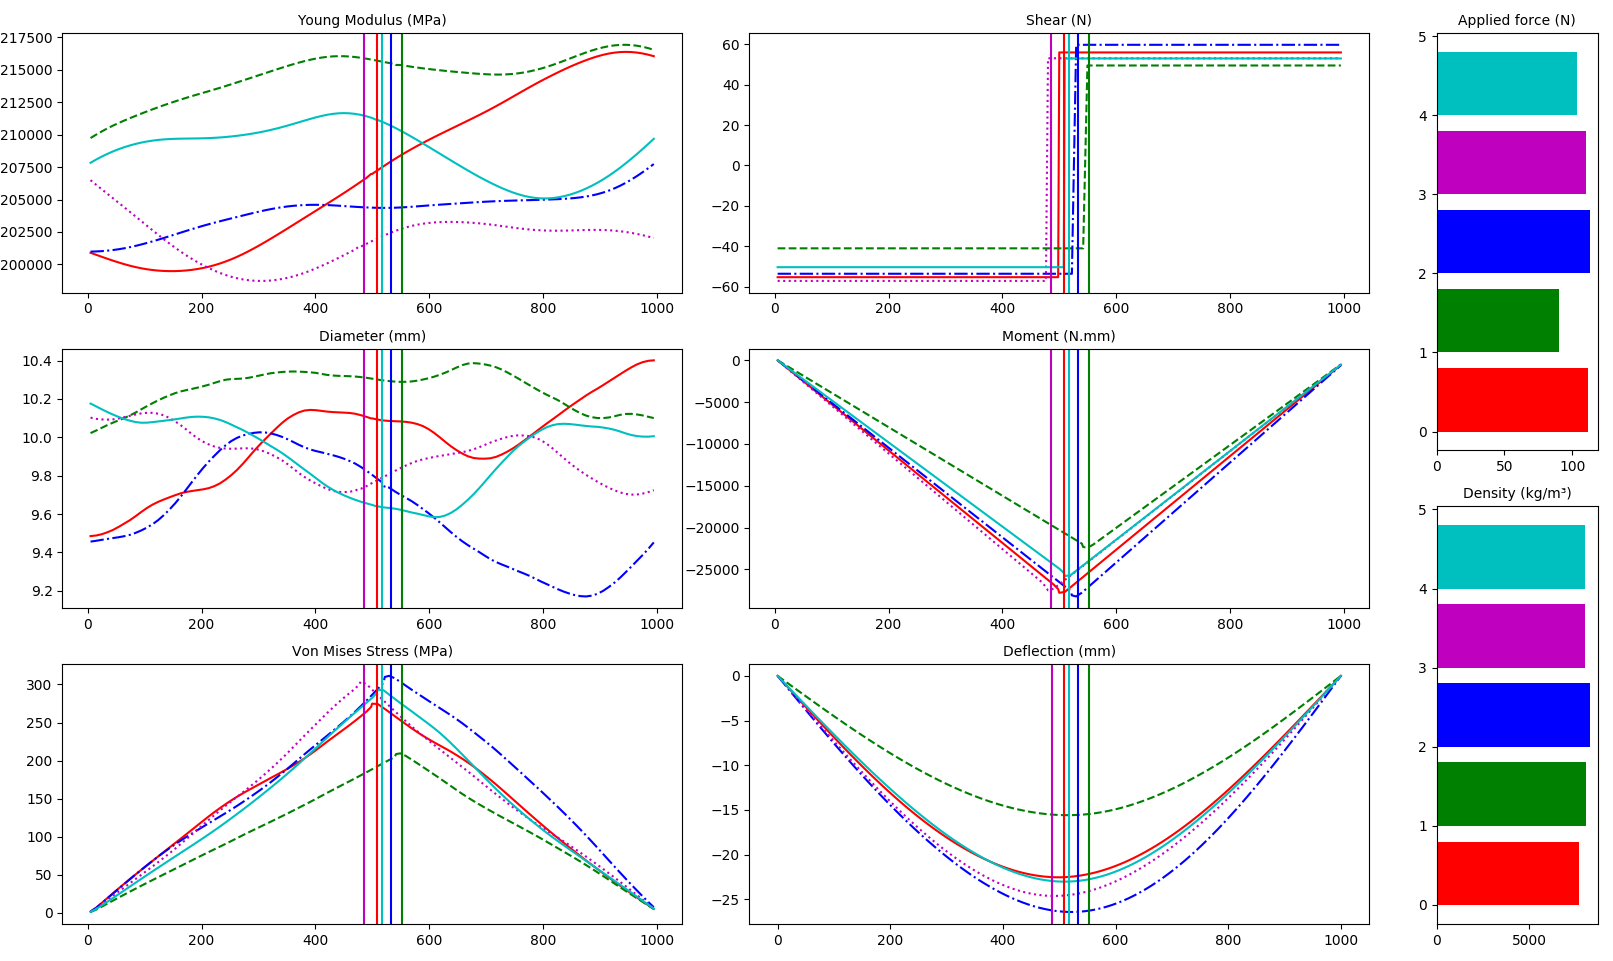
\includegraphics[scale=0.33]{beam_experience.png}
      \caption{Échantillon de 5 réalisations de la poutre en flexion. [Sur la gauche : Processus gouvernant le module de young, Processus gouvernant le diamètre, contrainte de Von Mises] | [Sur la droite : Contrainte de cisaillement, moment de flexion, déflexion] }
         \label{beamExperience}
\end{figure}

Les grandeurs d'étude choisies ici sont la contrainte de Von Mises, la déflection de chaque noeud, et la déflection maximale. On pourrait de même choisir une contrainte de Von Mises maximale pour représenter la défaillance. 

Comme chacun des processus stochastiques peut être décomposé en une somme finie de variables aléatoires normales grâce à la décomposition de karhunen-Loeve, l'on peut à l'inverse, générer des champs stochastiques à partir d'une collection de variables aléatoires, dont les paramètres sont issus de l'analyse même du champ.

On considère donc notre modèle plus comme fonction de variables aléatoires et de processus stochastiques, mais seulement comme une fonction de variables aléatoires scalaires.

Ceci permet de faire l'analyse de sobol classique (avec l'algorithme de sensibilité de \textit{Saltelli}) sur ces nouvelles variables aléatoires.

La difficultée ici, est d'ensuite relier les indices de sensiblité de Sobol des variables aléatoires définissant le champ au champ stochastique même. (On ne souhaite n'avoir qu'un seul indice de sobol pour un champ.) 

\subsection{Choix des codes et difficultées algorithmiques}
Au vu de choix de développer une méthode algorithmique pour l'analyse de sensiblité sur des champs stochastiques, et non pas de juste faire l'analyse de sensibilité sur une seule problématique, il y avait un besoin de robustesse supplémentaire pour l'écriture des différents codes. Ces derniers doivent pouvoir fonctionner avec tout type de fonction en python prennant en entrée des champs et variables aléatoire, et renvoyant un tuple de variables aléatoires. 

Pour pouvoir tester ceci, l'exemple de la poutre en éléments fins à été codée à part, et peut être utilisée directement comme fonction, indépendamment de l'analyse de sensibilité. Cette dernière prend de même en entrée deux champs stochastiques et trois variables aléatoires, et peut renvoyer plusieurs arguments. Les tests ont été faits avec la fonction ne renvoyant qu'une collection de champs (contraintes de von mises) et avec la fonction renvoyant un tuple (collection de champs + vecteur déflection maximale). Ce choix augmente le nombre de vérification qu'il y a à effectuer au sein du code, mais permet l'utilisation d'un plus grand nombre de fonctions, et l'analyse de sensiblité sur l'ensemble des variables de sortie en une seule fois.

Pour parvenir à bien controller les processus stochastiques, une classe a été écrite \textit{NdGaussianProcessConstructor}, qui permet de définir entièrement un processus stochastique, et possède de nombreuses méthodes pour créer des échantillons, faire les décompositions de Karhunen-Loeve, ou encore reconstituer un champ à partir de la dite décomposition. Enfin, comme les échantillons sont nécessaires pour la décomposition de Karhunen-Loeve, et que ceux-ci peuvent être de taille plutôt importante, ils sont enregistrés sous form de \textit{numpy.memmap} dans un fichier temporaire, pour relacher un peu de pression sur la mémoire vive.\\

En interne, le modèle fonction de champs stochastiques, passe par un wrapper qui fait qu'on peut la considerer comme seulement fonction de variables aléatoires gaussiennes. Cela permet d'utiliser les méthodes internes à openturns comme l'algorithme de Saltelli pour estimer les indices de sobol. \\

Néanmoins, pour pallier certaines difficultées comme les fonctions qui par moment renvoient des \textbf{\textit{np.nan}} (donc lorsqu'il y a eu une erreur), on passe d'abord par une étape de correction:  l'ensemble des valeurs de sortie contenant des \textit{nan} sont regénérées, et comme les entrées de l'étude sont des combinaison de deux ensembles de variables aléatoires A et B, toutes les autres permuttations des entrées ayant entrainé des erreurs sont supprimées et remplacées. Cette étape est éxpliquée en figure \ref{posprocessing} \

Les codes sont accessibles via \textit{\textbf{github}}: \\
\url{https://github.com/Kramer84/stochastic_process_analysis}

\begin{figure}[H]
   \centering   
   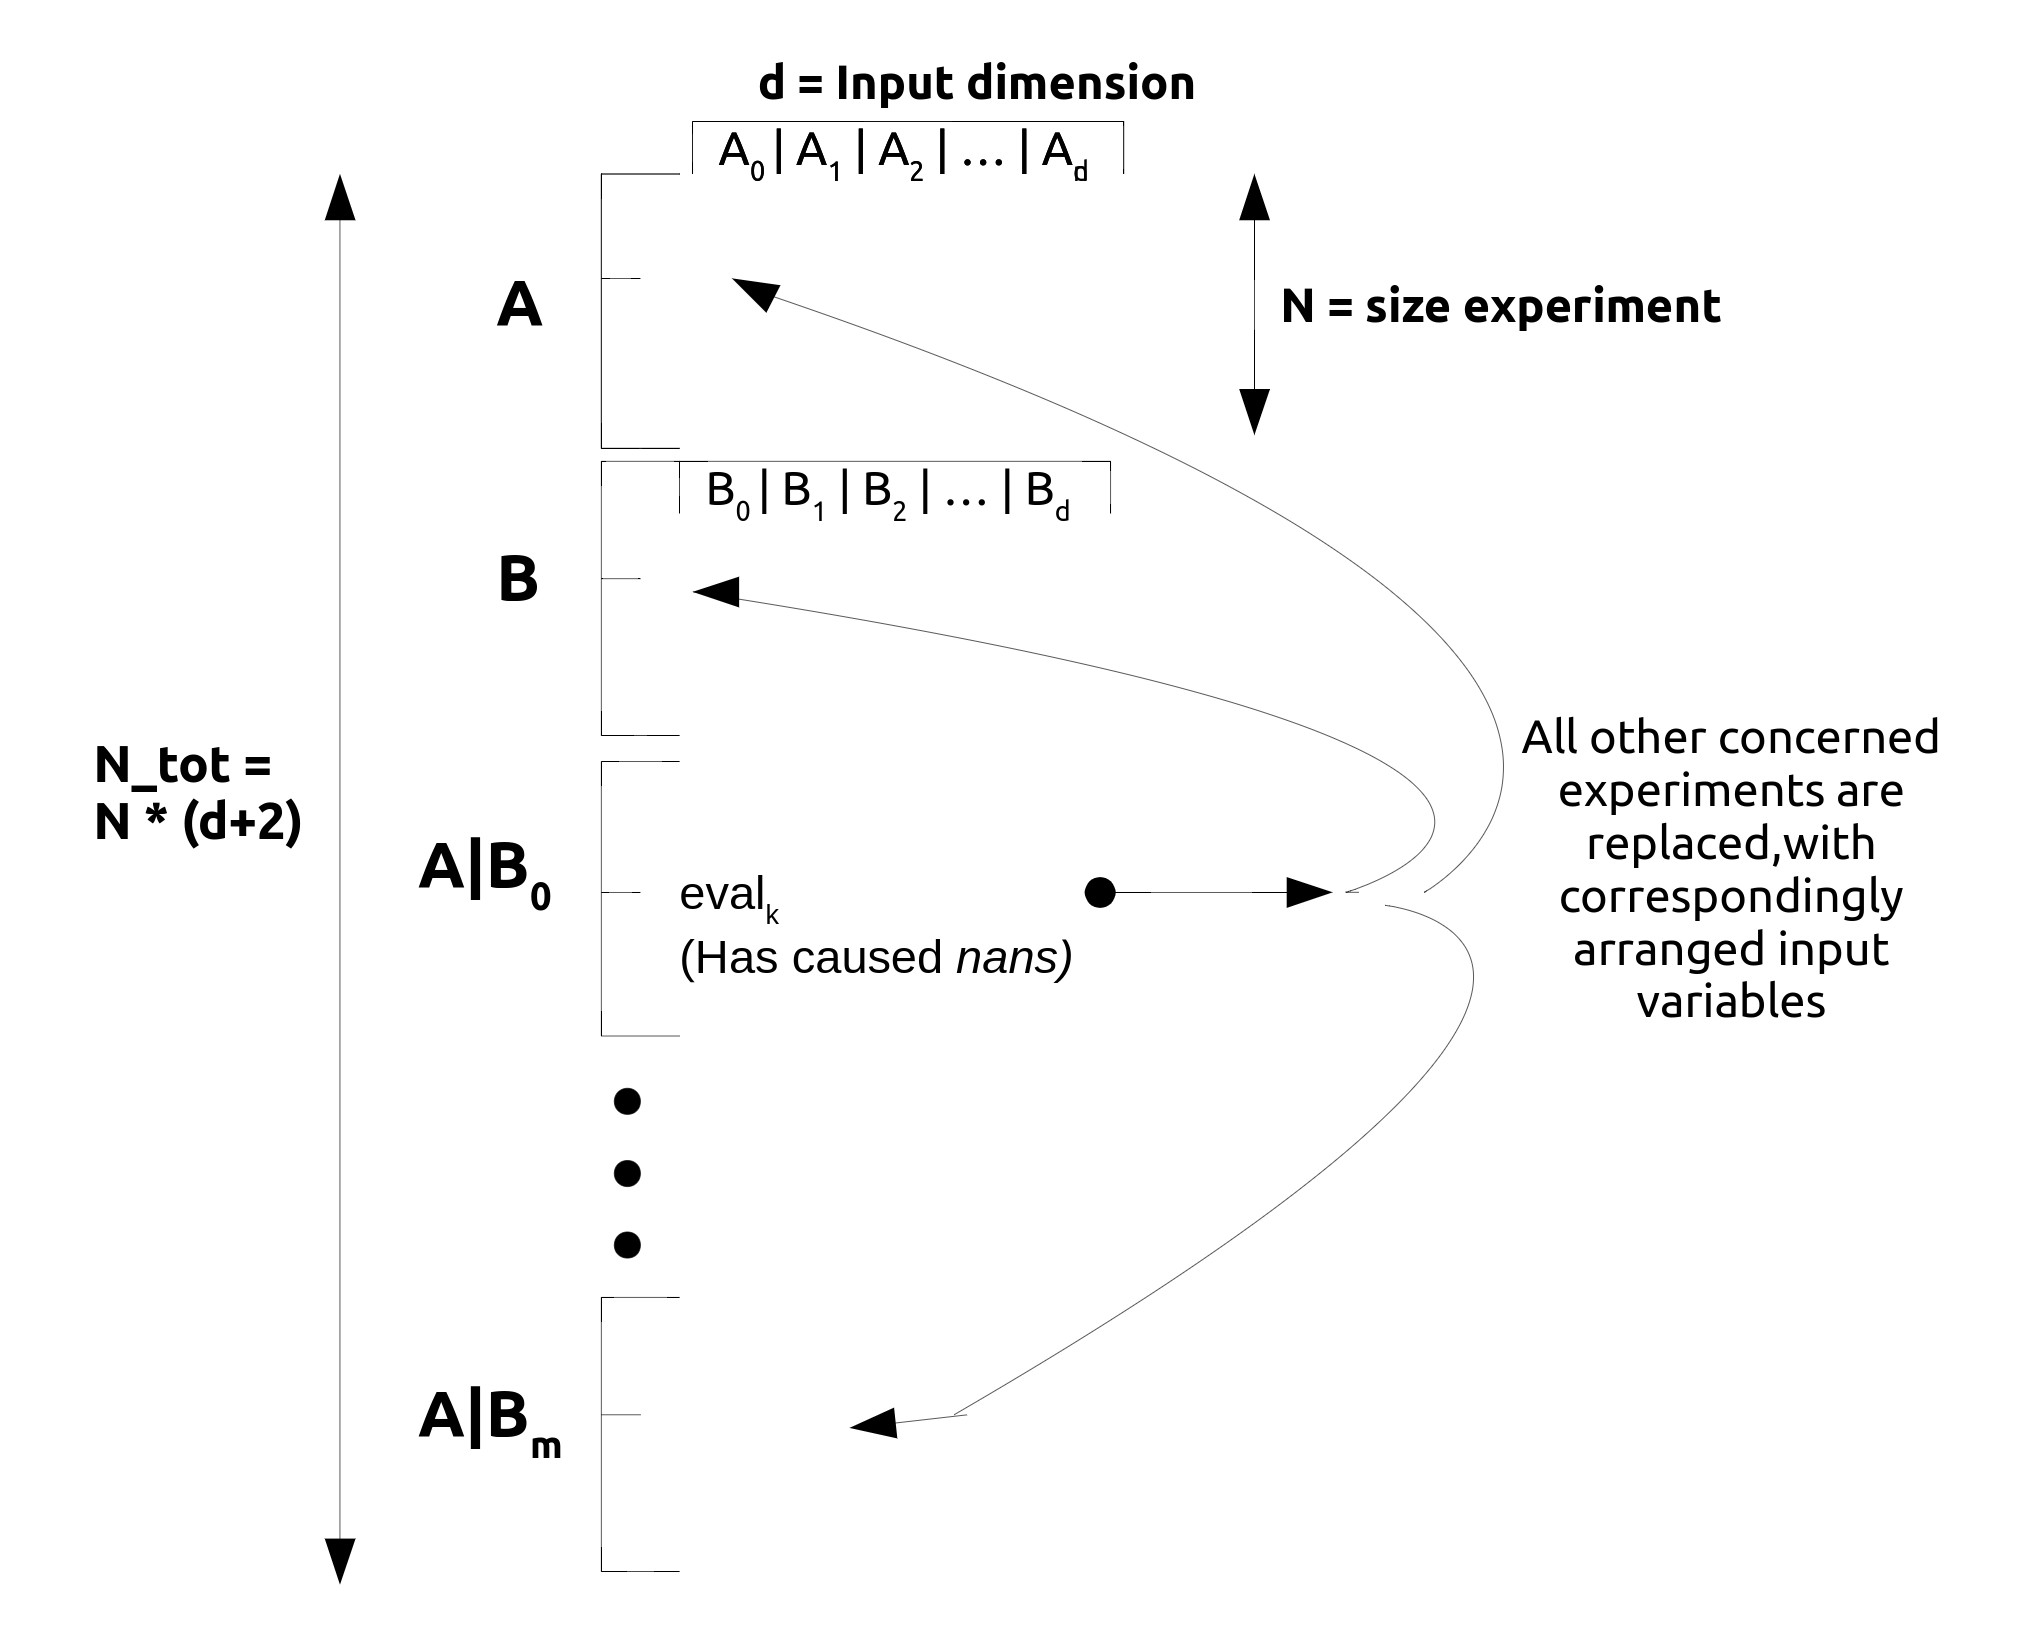
\includegraphics[scale=0.175]{schema_postprocessing.png}
      \caption{Organsiation des variables d'entrée, expliquant l'étape de postprocessing}
         \label{posprocessing}
\end{figure}


Une fois cette étape finie, on a accès aux indices de sobol pour chaque élément du champ. \\
Dans le cas de la poutre en flexion, prennant initialement 5 arguments en entrée (champ du module de young et champ du diamètre, densité, position de la force et norme de la force), la décomposition des deux champs en entrée fait que le modèle est ensuite régi par 24 variables aléatoires. Bien que cela fait augmenter la dimensionalité du problème, nous avons désormais la possiblité de travailler seuelement avec des variables aléatoires gaussiennes décorrélées, et donc faire une analyse de sensibilité classique.\\
La difficultée qui découle de cette analyse, est de trouver la manière qui permettra de relier les indices de sobol de ces variables aléatoire décorrélées, au champ stochastique d'origine. \\



\begin{figure}[H]
    \centering
    \begin{minipage}{0.45\textwidth}
        \centering
        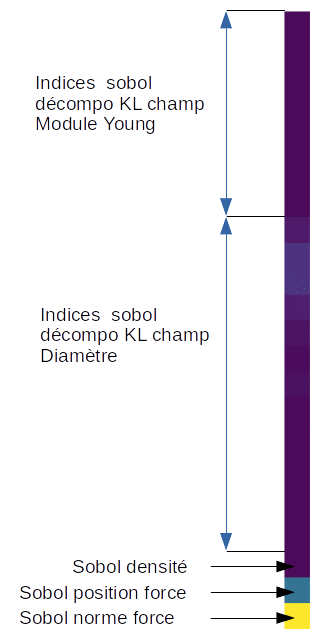
\includegraphics[height=1\textwidth]{sensitivity_rv_KL_anno.png} % first figure itself
        \caption{indices de sobol des V.A. de Karhunen-Loève pour la déflection maximale}
    \end{minipage}\hfill
    \begin{minipage}{0.45\textwidth}
        \centering
        
\includegraphics[width=1.35\textwidth]{sensitivity_field_KL.png} % second figure itself
        \caption{indices de sobol des V.A. de Karhunen-Loève pour le champ des contrainte de Von Mises}
    \end{minipage}
\end{figure}

Pour parvenir à faire ce lien, nous avions comme base différentes études sur le sujet, notamment le papier par \cite{Wei2017May}, sur l'analyse de sensibilité sur des modèles ayant des paramètres dépendants du temps. (Les variables étant gouvernées par le temps sont générallement stochastiques, ex: température, effort etc. ) \\

Mais ayant fait une analyse préliminaire de ces indices de sobol', des incohérences dans ces indices ont pu être remarqués. En effet, la somme de l'ensemble des indices du premier ordre doit être inferieure à 1 , et il ne peut y avoir d'indices négatifs. L'apparition d'indices de Sobol' négatifs peut être expliqué par un nombre d'experiences trop faible, nombre d'experiences qui lui même est limité par la mémoire disponible dans l'ordinateur. Néanmoins, ce n'était pas la seule incohérence. Nous vous présentons ici les indices de Sobol' pour la contrainte de Von Mises dans chaque élément de la poutre, et nous essayons de voir l'influence de l'augmentation du nombre d'experiences sur le nombre d'indices de Sobol' qui sont négatifs, ou voir comment varie la somme de l'ensemble des indices de Sobol' associés à un seul élément. Nous utilisons ici $N=100 , N=500, N=1000, N=2500$



\subsection{Premiers essais d'analyse de la sensibilité du modèle }

Comme nous avions désormais accès aux différents indices de sobol de notre modèle basé sur la décompostion de Karhunen-Loève, le travail pouvait désormais se focaliser sur l'interprétation de ces différents indices. En effet, cette décomposition était très classique lors du travail avec des champs stochastiques, et plusieurs papiers de recherche se sont interessés à comment faire des  analyses de sensibilité de ce type de champs avec cette même décomposition. Comme mentionné précédemment, le travail de \cite{Wei2017May} offre une première approche pour l'interprétration de ces résultats, mais d'autres comme \cite{Pronzato2019Jul} ont aussi developpés des méthodes pour l'analyse de ces indices issus de l'expansion de Karhunen-Loève. 
Dans le travail de \cite{shangStochastic2013}, il est rapporté d'une méthodologie pour lier un modèle en élément finis d'Abaqus avec des champs stochastiques genérés avec MATLAB et pour l'analyse probabiliste de ce modèle. L'utilisation de l'expansion de KL y est aussi mentionné, et ce travail offre une analyse intéressante sur la capacité de cette méthode à reproduire le champs stochastique, en fonction de l'élément à partir duquel on troncature cette expansion. 

%\subsubsection{Essais sur la réponse du champs stochastique à la variation individuelle des variables auxilliaires issues de l'expansion de Karhunen-Loève}
%Comme dans les différentes méthodes proposées on génère le champ stochastique à partir d'une réalisation de variables auxilliaires et que l'on retrouve la corréspondance grâce aux vecteurs et valeurs propres de la matrice de covariance, il convient d'observer empiriquement sur un champ stochastique classique sa réaction face aux changement dans les différentes variables auxilliaires. Dans les notations adoptées précédemment, cela vient à vérifier l'amplitude et la nature du changement dans le champ stochastique $Y_{i}$, lors de changement dans les variables $\left(\xi_{i1}, \ldots, \xi_{iM_{i}}\right)$. \\

%Soit $Y_{i}$ un champ stochastique ayant comme modèle de covariance celui de Matern, et des  


\subsubsection{Interprétation et essais avec le papier : "Time-variant global reliability sensitivity analysis of structures with both input random variables and stochastic processes"}
Ce papier de recherche datant de 2017, offre une approche pour l'analyse de sensibilité de modèles définis dans le temps et leur analyse de fiabilité. En effet, de nombreuses structures mécaniques (ponts, tours etc.) sont soumis à des grandeurs variant dans le temps, et si celles se trouvent être continues dans celui ci, alors cette grandeur peut être représentée par un champ stochastique. Bien qu'il y aie une différence notable entre les grandeurs par rapport auxquelles il y a continuité (dans leur papier le temps, et nous l'espace), des analogies peuvent être faites. \\

L'approche se base sur la décomposition de Karhunen-Loève du champ stochastique, permettant de considérer le problème comme uniquement dépendant de variables aléatoire gaussiennes décorrélées, et de déduire la sensibilité du modèle au champ stochastique à partir de la sensibilité de chaque composant de la décomposition du champ. \\ 

La décomposition de KL est particulièrement utile pour le calcul de fonction d'enveloppe et les calculs fiabilistes. Dans ce papier, l'utilisation de l'experience de Monte-Carlo est essentiellement utilisée pour être comparée aux autres méthodes développées (\textbf{FOEF} : First Order Envelope Function et \textbf{AK-MCS} Active learning Kriging based Monte Carlo Simulation).\\

L'utilité de cette approche est de pouvoir identifier les sources principales d'incertitude ayant le plus d'influence sur la fiabilité du modèle. Enfin, elle permet de classer les variables selon leur ordre d'influence. \\

Néanmoins, leur approche se base sur la définition d'un état limite du modèle (par exemple la différence entre la contrainte maximale et la contrainte limite) et d'une fonction indicatrice de l'état limite, alors que nous cherchons à évaluer la sensibilité d'une grandeur en sortie (par exemple la contrainte) par rapport aux variables aléatoire en entrée. Ceci revient à priori à mesurer l'impact qu'à une variables en entrée sur la variance de la grandeur en sortie. \\

La définition mathématique de leur problème est la suivante : 

%Approximation de Kahrunen Loeve 
   \[
      \begin{array}{lp{0.8\linewidth}}
         S             & : Etat limite du modèle \\
         \textbf{X}    & : Vecteur de variables aléatoire \\
         \textbf{Y}(t) & : Vecteur de champs stochastiques dépendants du temps \\
         \textbf{Z}    & : Fonction de performance \\
         I_S 	       & : Fonction indicatrice \\
         R  		   & : Probabilité de défaillance sur l'intervalle [0,T]
      \end{array}
   \]
   \begin{eqnarray}   
S = \left\lbrace \left( \textbf{X},\textbf{Y}\right) :Z(t)=g\left(\textbf{X},\textbf{Y}(t),t\right)<0\ \forall t \in\left[0,T \right] \right\rbrace ;\\
I_S(t) = I_S(\textbf{X},\textbf{Y}(t),T) = 
\begin{cases}
	1 &  (\textbf{X},\textbf{Y}) \in S \\ 
	0 &  (\textbf{X},\textbf{Y}) \not\in S
\end{cases}\ ;\\
R = R(T) = P_r(I_S=1) = Pr(Z(t) = g(\textbf{X},\textbf{Y}(t) < 0, \forall t \in \left[0,T\right]) \ ;
   \end{eqnarray}\\

Les variables aléatoire et champs stochastiques ici définis sont tous indépendants entre eux. \\

Soient $\mu_{X}=(\mu_{X_{1}},\ldots,\mu_{X_{n}})$ et $\sigma_{X}=(\sigma_{X_{1}},\ldots,\sigma_{X_{n}})$ les vecteurs des moyennes et écarts types des variables aléatoires et $\mu_{Y}=(\mu_{Y_{1}},\ldots,\mu_{Y_{n}})$ et $\sigma_{Y}=(\sigma_{Y_{1}},\ldots,\sigma_{Y_{n}})$ les vecteurs des moyennes et écarts types des champs stochastiques. \\

Comme explicité lors de la définition de la décomposition de Karhunen-Loève, tout champ stochastique $Y_{i}(t)$ peut être écrit comme une somme de variables aléatoire gaussiennes décorrélées. 
\[
	\begin{array}{lp{0.8\linewidth}}
		Y_{i}(t)		& Approx. Procéssus Gaussien $Y_{i}$ \\
		\lambda_{ik}	& Valeur Propre de la matrice de covariance \\
		\xi_{ik}		& Variable Normale Centrée Réduite \\
		\varphi_{ik}(t)	& Vecteur propre de la matrice de covariance
	\end{array}
\]
   \begin{eqnarray}
Y_{i}(t) & = & \mu_{Y_{i}}(t) +  \sum_{k=1}^{M}\sqrt{\lambda_{ik}}\xi_{ik}\varphi_{ik}(t);
   \end{eqnarray}\\

D'où chaque champ gaussien peut être exprimé à partir d'un ensemble de variables aléatoire gaussiennes décorélées $\xi_{i}=(\xi_{i1},\ldots,\xi_{iM_{i}})$ et l'ensemble des champs est représenté par le vecteur $\xi=(\xi_{1},\ldots,\xi_{m})$. $\xi_{i}$ étant la représentation par des variables auxilliaires du champ $Y_{i}$. 

Grâce à la propriété de décomposition de la variance, on a :

\begin{figure}[H]
   \centering   
   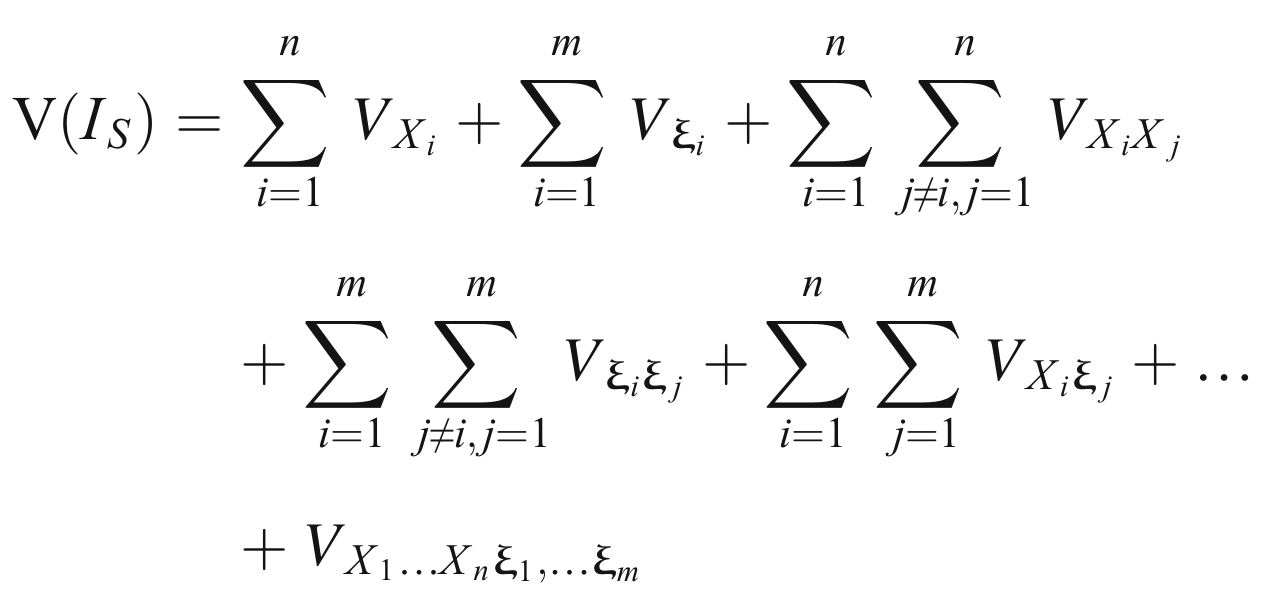
\includegraphics[scale=0.175]{DecompositionVariance.png}
      \caption{Decomposition de la variance de la fonction indicatrice}
         \label{VarDecompo}
\end{figure}

Ici, c'est la variance de la fonction indicatrice $I_{s}$ en sortie qui est traitée, mais ceci est faisable pour tout modèle dépendant d'un ensemble de variables aléatoire. Il est à remarquer ici que : 
$V_{X_{i}} = V\left[E\left(I_{S}|X_{i}\right)\right]$ qui est la variance conditionelle de la sortie $I_{S}$ lorsque la variable aléatoire $X_{i}$ est connue. \\ 
\\
Néanmoins, dans le cas du vecteur $\xi_{i} = (\xi_{i_{1}},\ldots,\xi_{i_{M_{i}}})$ on a: \\
\begin{eqnarray}
V_{\xi_{i}} = V\left[E\left(I_{S}|\xi_{i}\right)\right] = V\left[E\left(I_{S}|(\xi_{i_{1}},\ldots,\xi_{i_{M_{i}}})\right)\right] - \sum_{p=1}^{M_{i}}V_{\xi_{i_{p}}}
\end{eqnarray}
qui est la variance conditionelle de la sortie lorsque le vecteur aléatoire $\xi_{i}$ représentatif du champ stochastique $Y_{i}$ est connu.\\
\\  
Pour le calcul du vecteur des variances $V\left[E\left(I_{S}|(\xi_{i_{1}},\ldots,\xi_{i_{M_{i}}})\right)\right]$, dans le cadre d'une experience de Monte-Carlo, ceci pourrait se faire en rajoutant dans le plan d'experience, toutes les permutations associées à ces variables annexes aux champs stochastiques. \\

Avec le plan d'experience classique proposé par openTURNS, nous sommes en capacité de facilement calculer les indices de Sobol' du $1^{er}$ ordre de toutes les variables $S_{X_{i}}$ et $S_{\xi_{i_{p}}}$. Or nous cherchons $S_{\xi_{i}}$.\\
Dans le cas d'un modèle $F$, prenant en entrée un vecteur de champs stochastiques $Y = (Y_{1},\ldots,Y_{m})$ et un vecteur de variables aléatoires $X = (X_{1},\ldots,X_{n})$ et défini comme suit:  
\begin{align}
\omega = F(X,Y) &\  ,\omega \in \Re^{\aleph}
\end{align}


On peut définir une fonction $F^{'}$, utilisant la décomposition de Karhunen-Loève et seulement dépendante d'un ensemble de variables aléatoires décorrélées: 
\begin{align}
\omega = F^{'}(X,\xi) \\
\xi = (\xi_{1},\ldots,\xi_{m})\\
\xi_{i} = (\xi_{i_{1}},\ldots,\xi_{i_{M_{i}}})
\end{align} \\

Nous savons que : 
\begin{align}
V_{X_{i}} = V[E[\omega|X_{i}]] \\
S_{X_{i}} = \frac{V_{X_{i}}}{V(\omega)} \\
V_{X_{i}X_{j}} = V[E[\omega|X_{i}X_{j}]] - V_{X_{i}} - V_{X_{j}} \\
S_{X_{i}X_{j}} = \frac{1}{V(\omega)}V[E[\omega|X_{i}X_{j}]] - S_{X_{i}} - S_{X_{j}}
\end{align} \\

Néanmoins, à la différence des effets d'interactions et les sensibilités qui y sont associées, dans la cas de la sensibilité du champ stochastique, il semblerait qu'on ne soustraie pas l'effet de l'interaction du premier ordre, donc on n'aurait pas :
\begin{align}
S_{\xi_{i}} = S_{\xi_{i_{1}},\ldots,\xi_{i_{M_{i}}}} = \frac{1}{V(\omega)}V[E[\omega|\xi_{i_{1}},\ldots,\xi_{i_{M_{i}}}]] - \sum_{p=1}^{M_{i}}S_{\xi_{i_{p}}}
\end{align}

Mais plutôt seulement : 
\begin{align}
S_{\xi_{i}} = \frac{1}{V(\omega)}V[E[\omega|\xi_{i_{1}},\ldots,\xi_{i_{M_{i}}}]]
\end{align}

Ceci est intéressant dans la sens ou cela diminue grandement la complexité du calcul et qu'il ne faut plus que calculer les effets d'interaction et non plus les indices de sobol du premier ordre associés aux indices de KL des champs stochastiques. 

%Néanmoins dans le méthode présentée par \cite{Wei2017May}, on n'y fait pas mention d'une permutation de toutes les colonnes associées à un champ stochastique pour calculer l'effet d'interaction. Ceci fait supposer qu'il existe une autre manière d'arriver à trouver ces effet d'interaction, sans passer par cette permutation lors de l'experience de monte carlo ou que le calcul de cette interaction semblait trop triviale pour être mentionnée dans le papier:\\

%\begin{quote}
%\cite{Wei2017May}:\  By subtracting the first order partial variance $V_{X_{i}}$ and $V_{X_{j}}$ from $V[E(I_{S}|X_{i}, X_{j})]$, the second order partial variance $V_{X_{i}X_{j}}$ quantifies the second order interaction contribution between $X_{i}$ and $X_{j}$ to R. Similarly, $V_{\xi_{i}\xi_{j}}$ quantifies the second order interaction contribution between the stochastic process $Y_{i}(t)$ and $Y_{j}(t)$ to R, and $V_{X_{i}\xi_{j}}$ measures the second order interaction effect of the random variable $X_{i}$ and the stochastic process $Y_{j}(t)$ to R. \textbf{\textit{Higher order effect indices can be similarly defined and interpreted.}}
%\end{quote}

Le calcul à posteriori de ces interactions est possible, vu que nous n'avons qu'à comparer la moyenne des variance des deux échantillons de départ (\textbf{A} et \textbf{B}) à celle lorsque tout les paramètres du champs stochastique i sont connus ($V_{\xi_{i}}$). \\

Néanmoins, l'on ne peut pas inclure celles-ci dans le plan d'experience utilisé par openTURNS, vu que l'algorithme utilisé pour calculer les indices de Sobol' n'est concu que pour les calculs des indices de premier et second ordre de modèles gouvernés par un ensemble de variables aléatoires unitaires, et non des champs stochastiques. Pour parvenir à passer outre cette difficulté, un choix d'algorithme doit être fait pour le calcul de ces indices de sobol d'ordre fortement superieur. (Vu que pour les indices d'ordre 1, le choix de l'algorithme est entièrement libre.) Au vu du travail fait par PHIMECA sur l'analyse des lois asymptotiques des estimateurs des indices de Sobol \cite{dumas2017} ,l'on prendra comme estimateur celui de Martinez, mais il sera évidemment possible de rajouter à posteriori les autres estimateurs dans le workflow. \\ 

D'autre part, pour parvenir à garder cette complexité faible, nous sommes obligés de revoir la manière dont est fait le plan d'experience (la manière dont on mélange les différentes colonnes de nos deux samples \textbf{A} et \textbf{B}) puisque dans le cas de l'exemple de la poutre, nous aurions jusqu'a 5 fois moins de calculs à effectuer qu'en gardant tout les indices inutiles. \\
\begin{figure}[H]
   \centering   
   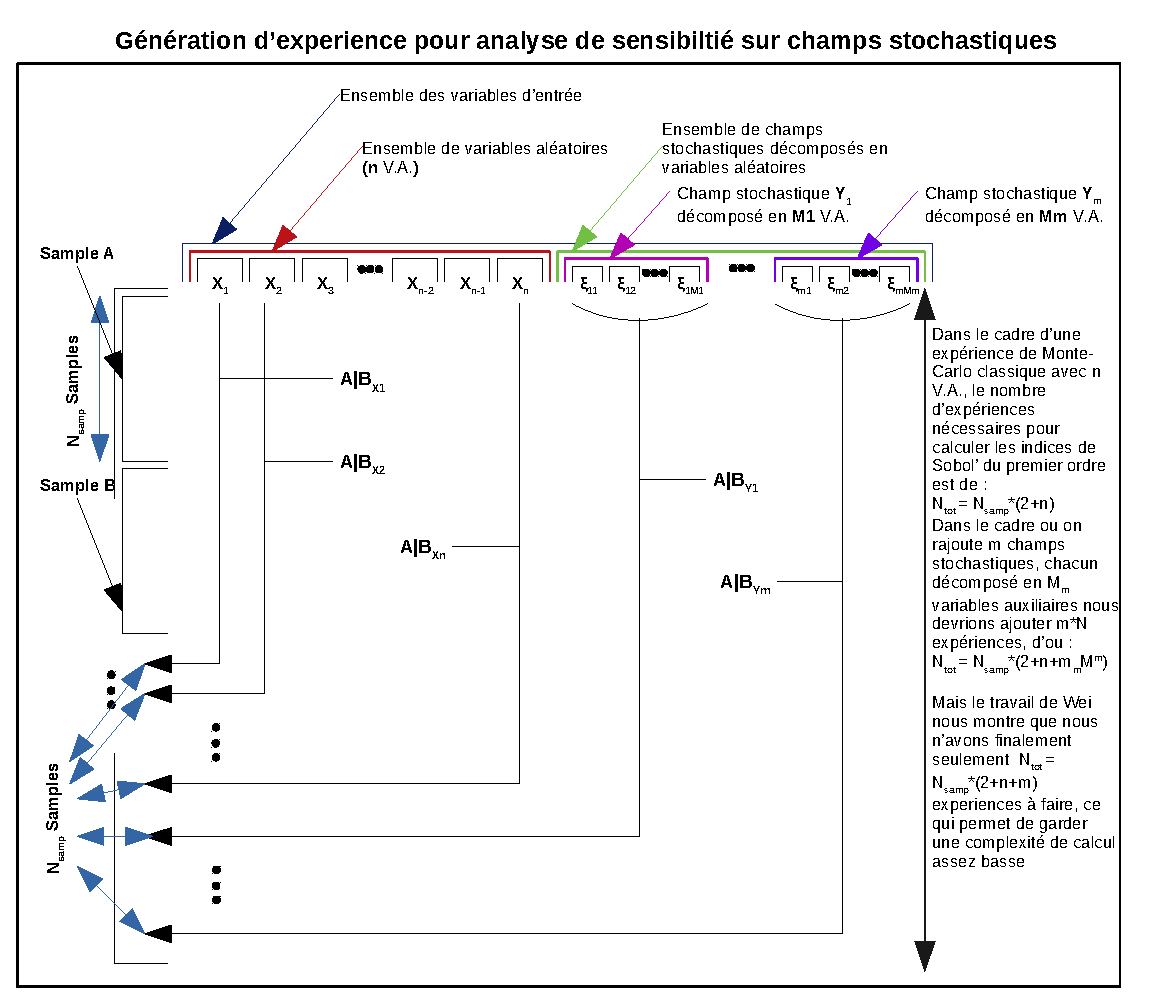
\includegraphics[scale=0.75]{Schema_Preparation_VA.pdf}
      \caption{Génération d’experience pour analyse de sensibiltié sur champs stochastiques}
         \label{expGenStoField}
\end{figure}
Les échantillons sont mélangés comme montré en figure \ref{expGenStoField}. 
Pour générer les samples de manière plus efficace, et être sur de couvrir l'ensemble du domaine de variance des lois d'entrée, est inclu dans le code la possibilité de générer l'échantillon en utlisant soit l'échantillonage LHS (Latin Hypercube Sampling), soit les séries à faible divergence (Low discrepancy series), soit une version optimisée du LHS (Simulated Annealing LHS). Bien sûr une génération entièrement aléatoire reste l'option de base.\\

Pour le calcul formel de l'estimateur de Sobol', nous allons utilisons la méthode par Saltelli, détaillée dans le papier par \cite{dumas2017}. Ce papier détail aussi la manière de calculer l'erreur dans le calcul de l'estimateur, paramètre important pour connaître la pertinence de l'estimateur. 



\subsection{Example of verbatim text}

\begin{verbatim}
        PROGRAM area
        REAL base, height, area
        PRINT *,'Enter the values for the base and height of a triangle.'
        READ *, base, height
        area = (1.0/2.0) * base * height
        PRINT *,'The area of a triangle with base ', base
        PRINT *,'and height ', height,' is ', area
        STOP
        END
\end{verbatim}

\paragraph{Note:}
In \texttt{verbatim} mode you can easily end up outside the
margins, as in the example above: pay attention to that!

\subsection{Lists}
Example of a list with numbered items:

   \begin{enumerate}
      \item  Planets, asteroids, moons \ldots
      \item  Stars, galaxies, quasars
  \end{enumerate}

Example of a list with unnumbered items:

   \begin{itemize}
      \item  Planets, asteroids, moons \ldots
      \item  Stars, galaxies, quasars
          
   \end{itemize}

\section{Results}

\newpage
\section{Tables and figures}




\begin{table}[htb]
      \caption[]{Example of table caption: opacity sources.}
         \label{KapSou}
     $$ 
         \begin{array}{p{0.7\linewidth}l}
            \hline
            \noalign{\smallskip}
            Source      &  T / {[\mathrm{K}]} \\
            \noalign{\smallskip}
            \hline
            \noalign{\smallskip}
            Yorke 1979, Yorke 1980a & \leq 1700           \\
            Kr\"ugel 1971           & 1700 \leq T \leq 5000 \\
            Cox \& Stewart 1969     & 5000 \leq             \\
            \noalign{\smallskip}
            \hline
         \end{array}
     $$ 
\end{table}

\section{Discussion}

\section{Conclusions}



% TABLES

\bibliography{Bibliographie_rapport_PHIMECA_Simady}


\end{document}

